\documentclass[12pt,a4paper]{article}

% ============================================================
% PACOTES
% ============================================================
\usepackage[utf8]{inputenc}
\usepackage[T1]{fontenc}
\usepackage[brazilian]{babel}
\usepackage{amsmath,amssymb}
\usepackage{graphicx}
\usepackage{booktabs}
\usepackage{caption}
\usepackage{float}
\usepackage{geometry}
\usepackage{hyperref}
\usepackage{xcolor}
\usepackage{enumitem}
\usepackage{array}
\usepackage{longtable}

\geometry{margin=2.5cm}
\hypersetup{
    colorlinks=true,
    linkcolor=blue,
    citecolor=blue,
    urlcolor=blue
}

% ------------------------------------------------------------
% Ambiente para indicar onde cada figura/imagem deve entrar,
% sem inserir a imagem de fato. Basta trocar o conteúdo do
% \fbox por \includegraphics{caminho/da/imagem.png} depois.
% (Nomes de arquivo usam hífen, nunca underscore, para não
% quebrar a compilação em modo texto normal do LaTeX.)
% ------------------------------------------------------------
\newcommand{\figuraPendente}[3]{%
\begin{figure}[H]
    \centering
    \fbox{\begin{minipage}{0.85\textwidth}
        \centering
        \vspace{2.5cm}
        \textbf{[INSERIR FIGURA AQUI]}\\[0.3cm]
        \textit{Arquivo sugerido:} \texttt{#1}\\[0.3cm]
        \textit{Conteúdo:} #2
        \vspace{2.5cm}
    \end{minipage}}
    \caption{#3}
    \label{fig:#1}
\end{figure}
}

% ============================================================
% CABEÇALHO / TÍTULO
% ============================================================
\title{
    \Large \textbf{Avanços em Inteligência Artificial} \\
    \large EELT7025 --- PPGEE, UFPR \\[0.3cm]
    \normalsize Exercícios da Aula 03 \\
    \normalsize Análise Exploratória de Dados (EDA)
}
\author{Adriely Teixeira de Paula, Betina Zynger Capaverde, Emilio Gaudeda Junior}
\date{\today}

% ============================================================
\begin{document}

\maketitle
\tableofcontents
\newpage

% ============================================================
\section*{Dataset utilizado}
\addcontentsline{toc}{section}{Dataset utilizado}

Os dois exercícios desta lista retomam, sobre \textbf{um único dataset real}, o roteiro completo de EDA: qualidade dos dados $\rightarrow$ univariada $\rightarrow$ outliers $\rightarrow$ tendência/sazonalidade (\textbf{Exercício 1}) $\rightarrow$ padrões cíclicos $\rightarrow$ autocorrelação $\rightarrow$ frequência $\rightarrow$ estacionariedade $\rightarrow$ relações bivariadas/multivariadas $\rightarrow$ anomalias (\textbf{Exercício 2}).

\textbf{Dataset:} \emph{PJM Hourly Energy Consumption} --- carga horária (MW) da região \textbf{PJME} (variável-alvo) e da região \textbf{PJMW} (variável exógena numérica, região vizinha da mesma malha elétrica). Período: 2002--2018.

\newpage
% ============================================================
% EXERCÍCIO 1
% ============================================================
\section{Exercício 1: Qualidade, Distribuição, Outliers e Tendência/Sazonalidade}

\subsection{Carregamento e período coberto}

\begin{table}[H]
\centering
\caption{Resumo do carregamento dos dados}
\begin{tabular}{lccc}
\toprule
Série & Nº de registros & Início & Fim \\
\midrule
PJME (alvo)     & 145.366 & 2002-01-01 01:00 & 2018-08-03 00:00 \\
PJMW (exógena)  & 143.206 & 2002-04-01 01:00 & 2018-08-03 00:00 \\
\bottomrule
\end{tabular}
\end{table}

\subsection{Checklist de qualidade dos dados}

\begin{itemize}
    \item \textbf{(a) Timestamps duplicados:} 4 duplicatas, concentradas em início de novembro às 02:00, artefato do horário de verão (DST \emph{fall-back}) nos EUA.
    \item \textbf{(b) Timestamps ausentes:} 30 lacunas no índice horário completo, concentradas em março/abril às 02:00--03:00, horas que ``somem'' no DST \emph{spring-forward}.
    \item \textbf{(c) Plausibilidade de escala/unidade:} PJME entre 14.544 e 62.009 MW, média 32.080 MW, nenhum valor negativo ou nulo suspeito.
    \item \textbf{(d) Hipótese sobre o mecanismo dos dados ausentes:} as 30 lacunas seguem um padrão perfeitamente previsível (mesma hora, mesmo dia do ano, todo ano), determinado por uma regra de calendário externa e não relacionado ao valor da própria demanda, caracteriza um mecanismo \textbf{MCAR} (\emph{Missing Completely At Random}).
    \item \textbf{(e) Variáveis categóricas:} o arquivo bruto não traz nenhuma coluna categórica; variáveis como \texttt{tipo\_dia} e \texttt{estacao} são derivadas do índice temporal no Exercício 2.
    \item \textbf{Tratamento aplicado:} reindexação para frequência horária completa + interpolação linear das lacunas. Série final: 145.392 observações, 0 ausentes, 0 duplicatas ($\approx$16,6 anos).
\end{itemize}

\subsection{Análise univariada, assimetria, curtose, CV e teste de normalidade}

\begin{table}[H]
\centering
\caption{Estatísticas descritivas: Carga PJME (MW)}
\begin{tabular}{lc}
\toprule
Estatística & Valor \\
\midrule
Média / Mediana        & 32.078,9 / 31.420,0 MW \\
Desvio-padrão          & 6.464,3 MW \\
Coeficiente de Variação (CV) & 0{,}2015 (20{,}2\%) \\
Assimetria (\emph{skew})     & 0{,}739 \\
Curtose (excesso)     & 0{,}736 \\
\bottomrule
\end{tabular}
\end{table}

\begin{table}[H]
\centering
\caption{Testes de normalidade}
\begin{tabular}{lcc}
\toprule
Teste & Estatística & $p$-valor \\
\midrule
D'Agostino-Pearson (N completo, $n$=145.392) & 12.473,9 & $<10^{-300}$ \\
Shapiro-Wilk (amostra de 5.000)              & 0{,}9675 & $3{,}63\times10^{-32}$ \\
\bottomrule
\end{tabular}
\end{table}

\noindent Ambos os testes rejeitam fortemente $H_0$ (normalidade), esperado tanto pela assimetria positiva quanto pelo tamanho da amostra (N muito grande torna os testes extremamente sensíveis a pequenos desvios da normalidade).

\begin{figure}[H]
    \centering
    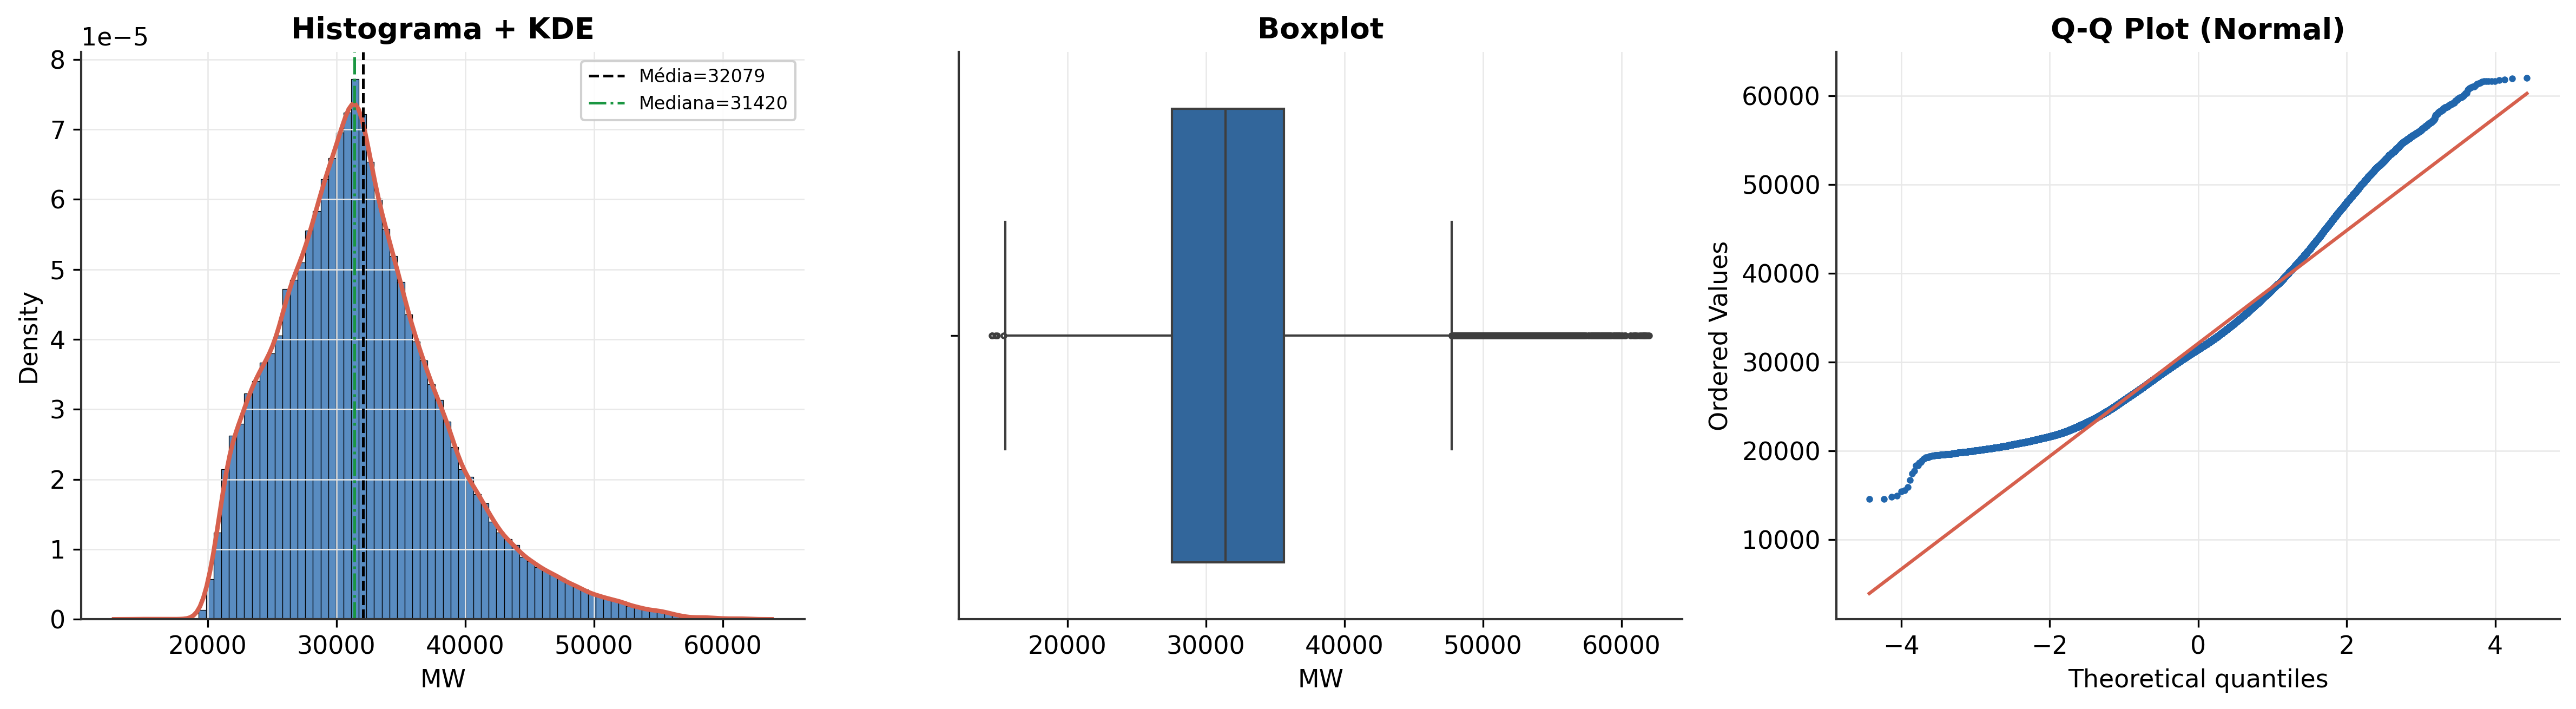
\includegraphics[width=0.85\textwidth]{Figuras_Aula3/fig1-histograma-boxplot-qqplot.png}
    \caption{Análise univariada da carga PJME: histograma, boxplot e Q-Q Plot.}
    \label{fig:fig1}
\end{figure}

\subsection{Outliers: IQR vs. Z-score Modificado (MAD): ruído ou anomalia real?}

\begin{table}[H]
\centering
\caption{Comparação de métodos de detecção de outliers}
\begin{tabular}{lcc}
\toprule
Método & Nº de outliers & \% dos dados \\
\midrule
IQR (limites [15.457, 47.761] MW) & 3.460 & 2{,}380\% \\
Z-score Modificado (MAD, $|Z_{mod}|>3{,}5$) & 1.003 & 0{,}690\% \\
\midrule
Sinalizados por ambos os métodos & \multicolumn{2}{c}{1.003} \\
\bottomrule
\end{tabular}
\end{table}

\begin{table}[H]
\centering
\caption{Distribuição mensal dos outliers de consenso (ambos os métodos)}
\begin{tabular}{lccccc}
\toprule
Mês & Maio & Junho & Julho & Agosto & Setembro \\
\midrule
Nº de pontos & 3 & 123 & 527 & 321 & 29 \\
\bottomrule
\end{tabular}
\end{table}

\begin{figure}[H]
    \centering
    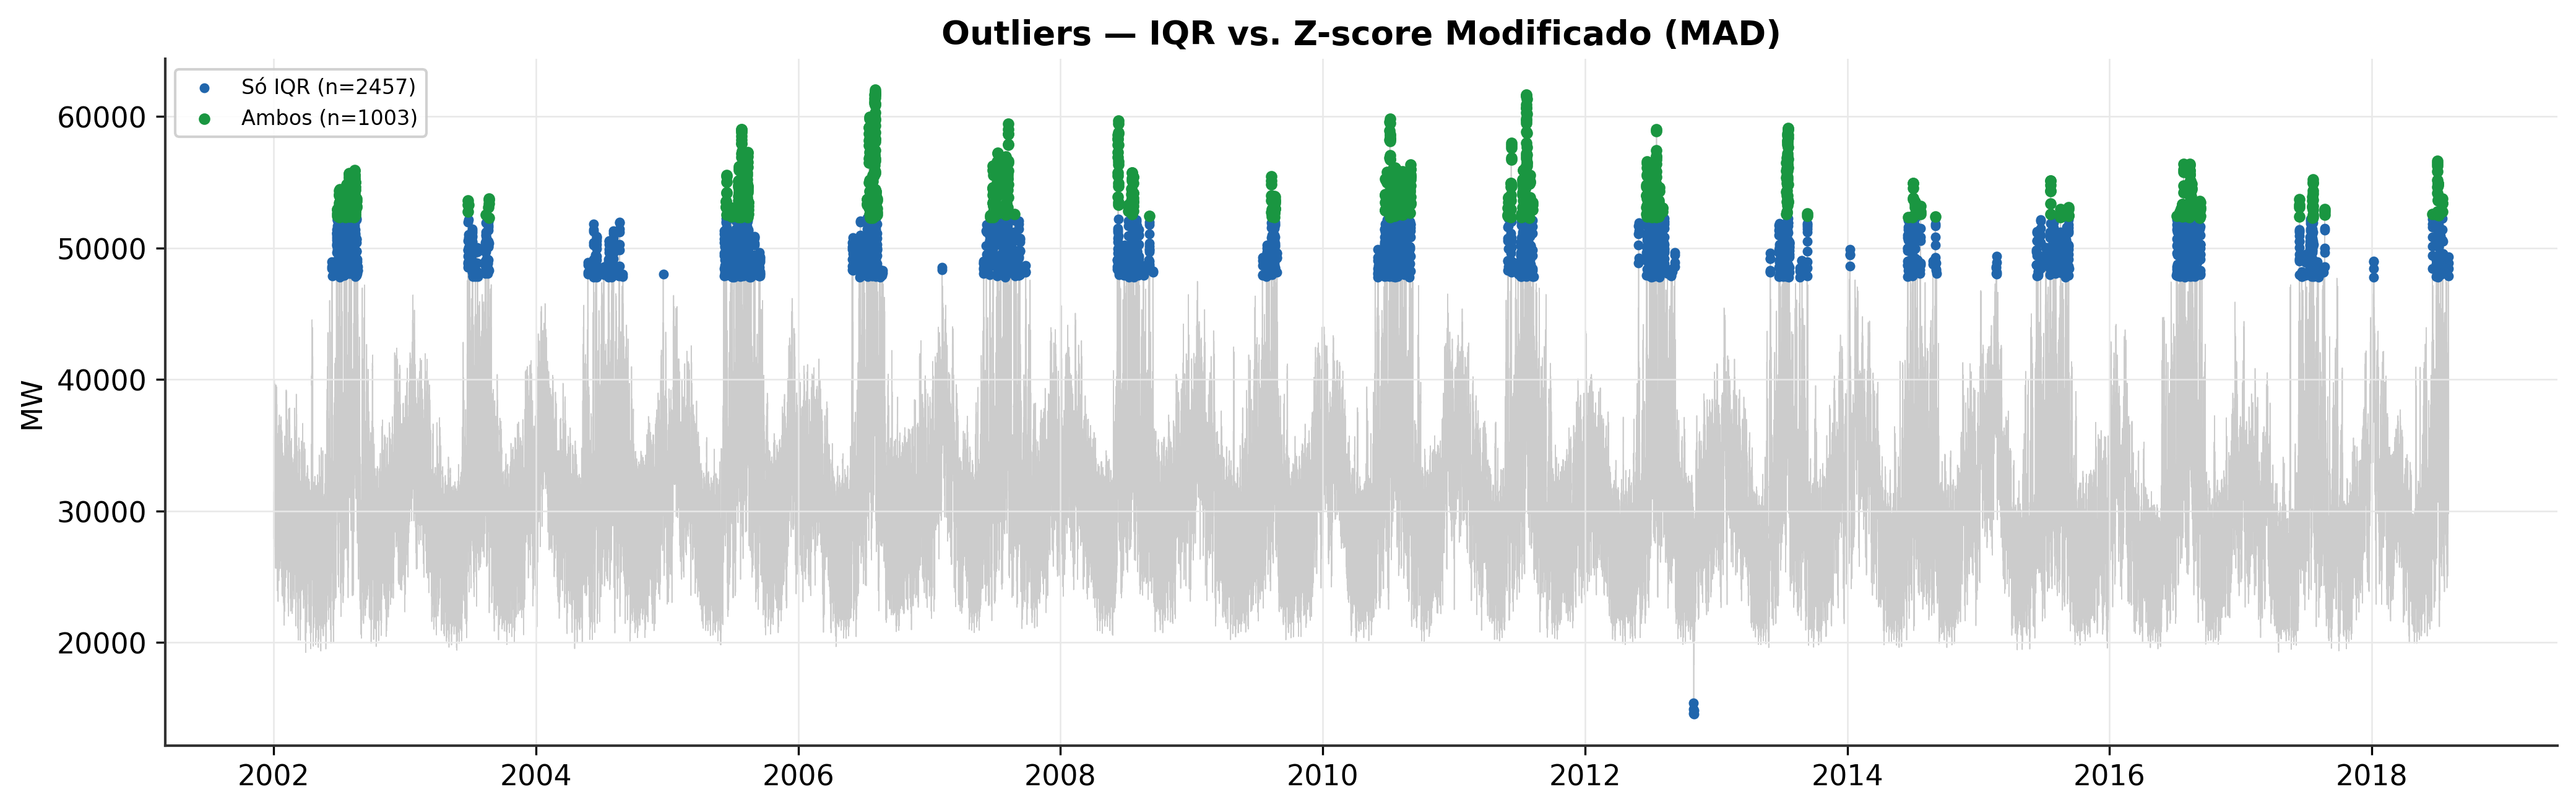
\includegraphics[width=0.85\textwidth]{Figuras_Aula3/fig2-outliers-iqr-mad.png}
    \caption{Outliers detectados: IQR vs. Z-score Modificado (MAD).}
    \label{fig:fig1}
\end{figure}


\subsubsection*{Ruído ou anomalia real?}
Os outliers de consenso concentram-se \textbf{exclusivamente nos meses de maio a setembro}, com pico acentuado em julho (527 pontos) e agosto (321 pontos), exatamente o período de maior estresse térmico por calor nos EUA. Isso é consistente com \textbf{anomalias reais de demanda} (picos de refrigeração em ondas de calor), não com ruído de medição: os valores são fisicamente plausíveis, persistem por várias horas/dias consecutivos (não são picos isolados de 1 amostra, típicos de erro de sensor) e coincidem com o período climático esperado. Notavelmente, o método de consenso \textbf{não} sinalizou picos de inverno (ondas de frio) como outliers, o MAD, mais conservador, aparentemente absorve a variação de inverno como parte da faixa "normal" de variação, sinalizando como anômalos apenas os extremos de calor do verão.

\subsection{Decomposição STL e Forças de Tendência/Sazonalidade}

\begin{table}[H]
\centering
\caption{STL, variância explicada por componente (sazonalidade diária, \texttt{period=24})}
\begin{tabular}{lcc}
\toprule
Componente & Variância & \% da var. total \\
\midrule
Tendência    & 19.418.383 & 46{,}5\% \\
Sazonalidade & 18.965.600 & 45{,}4\% \\
Resíduo      &  2.756.443 &  6{,}6\% \\
\bottomrule
\end{tabular}
\end{table}

\noindent Força de Tendência $F_T = 0{,}8850$ \quad|\quad Força de Sazonalidade $F_S = 0{,}8660$.

\noindent $F_S$ muito alta indica um ciclo diário extremamente forte e regular (rotina humana/industrial). $F_T$ moderada/alta indica que a variação sazonal de médio prazo (verão/inverno) também é relevante frente ao ruído residual.


\begin{figure}[H]
    \centering
    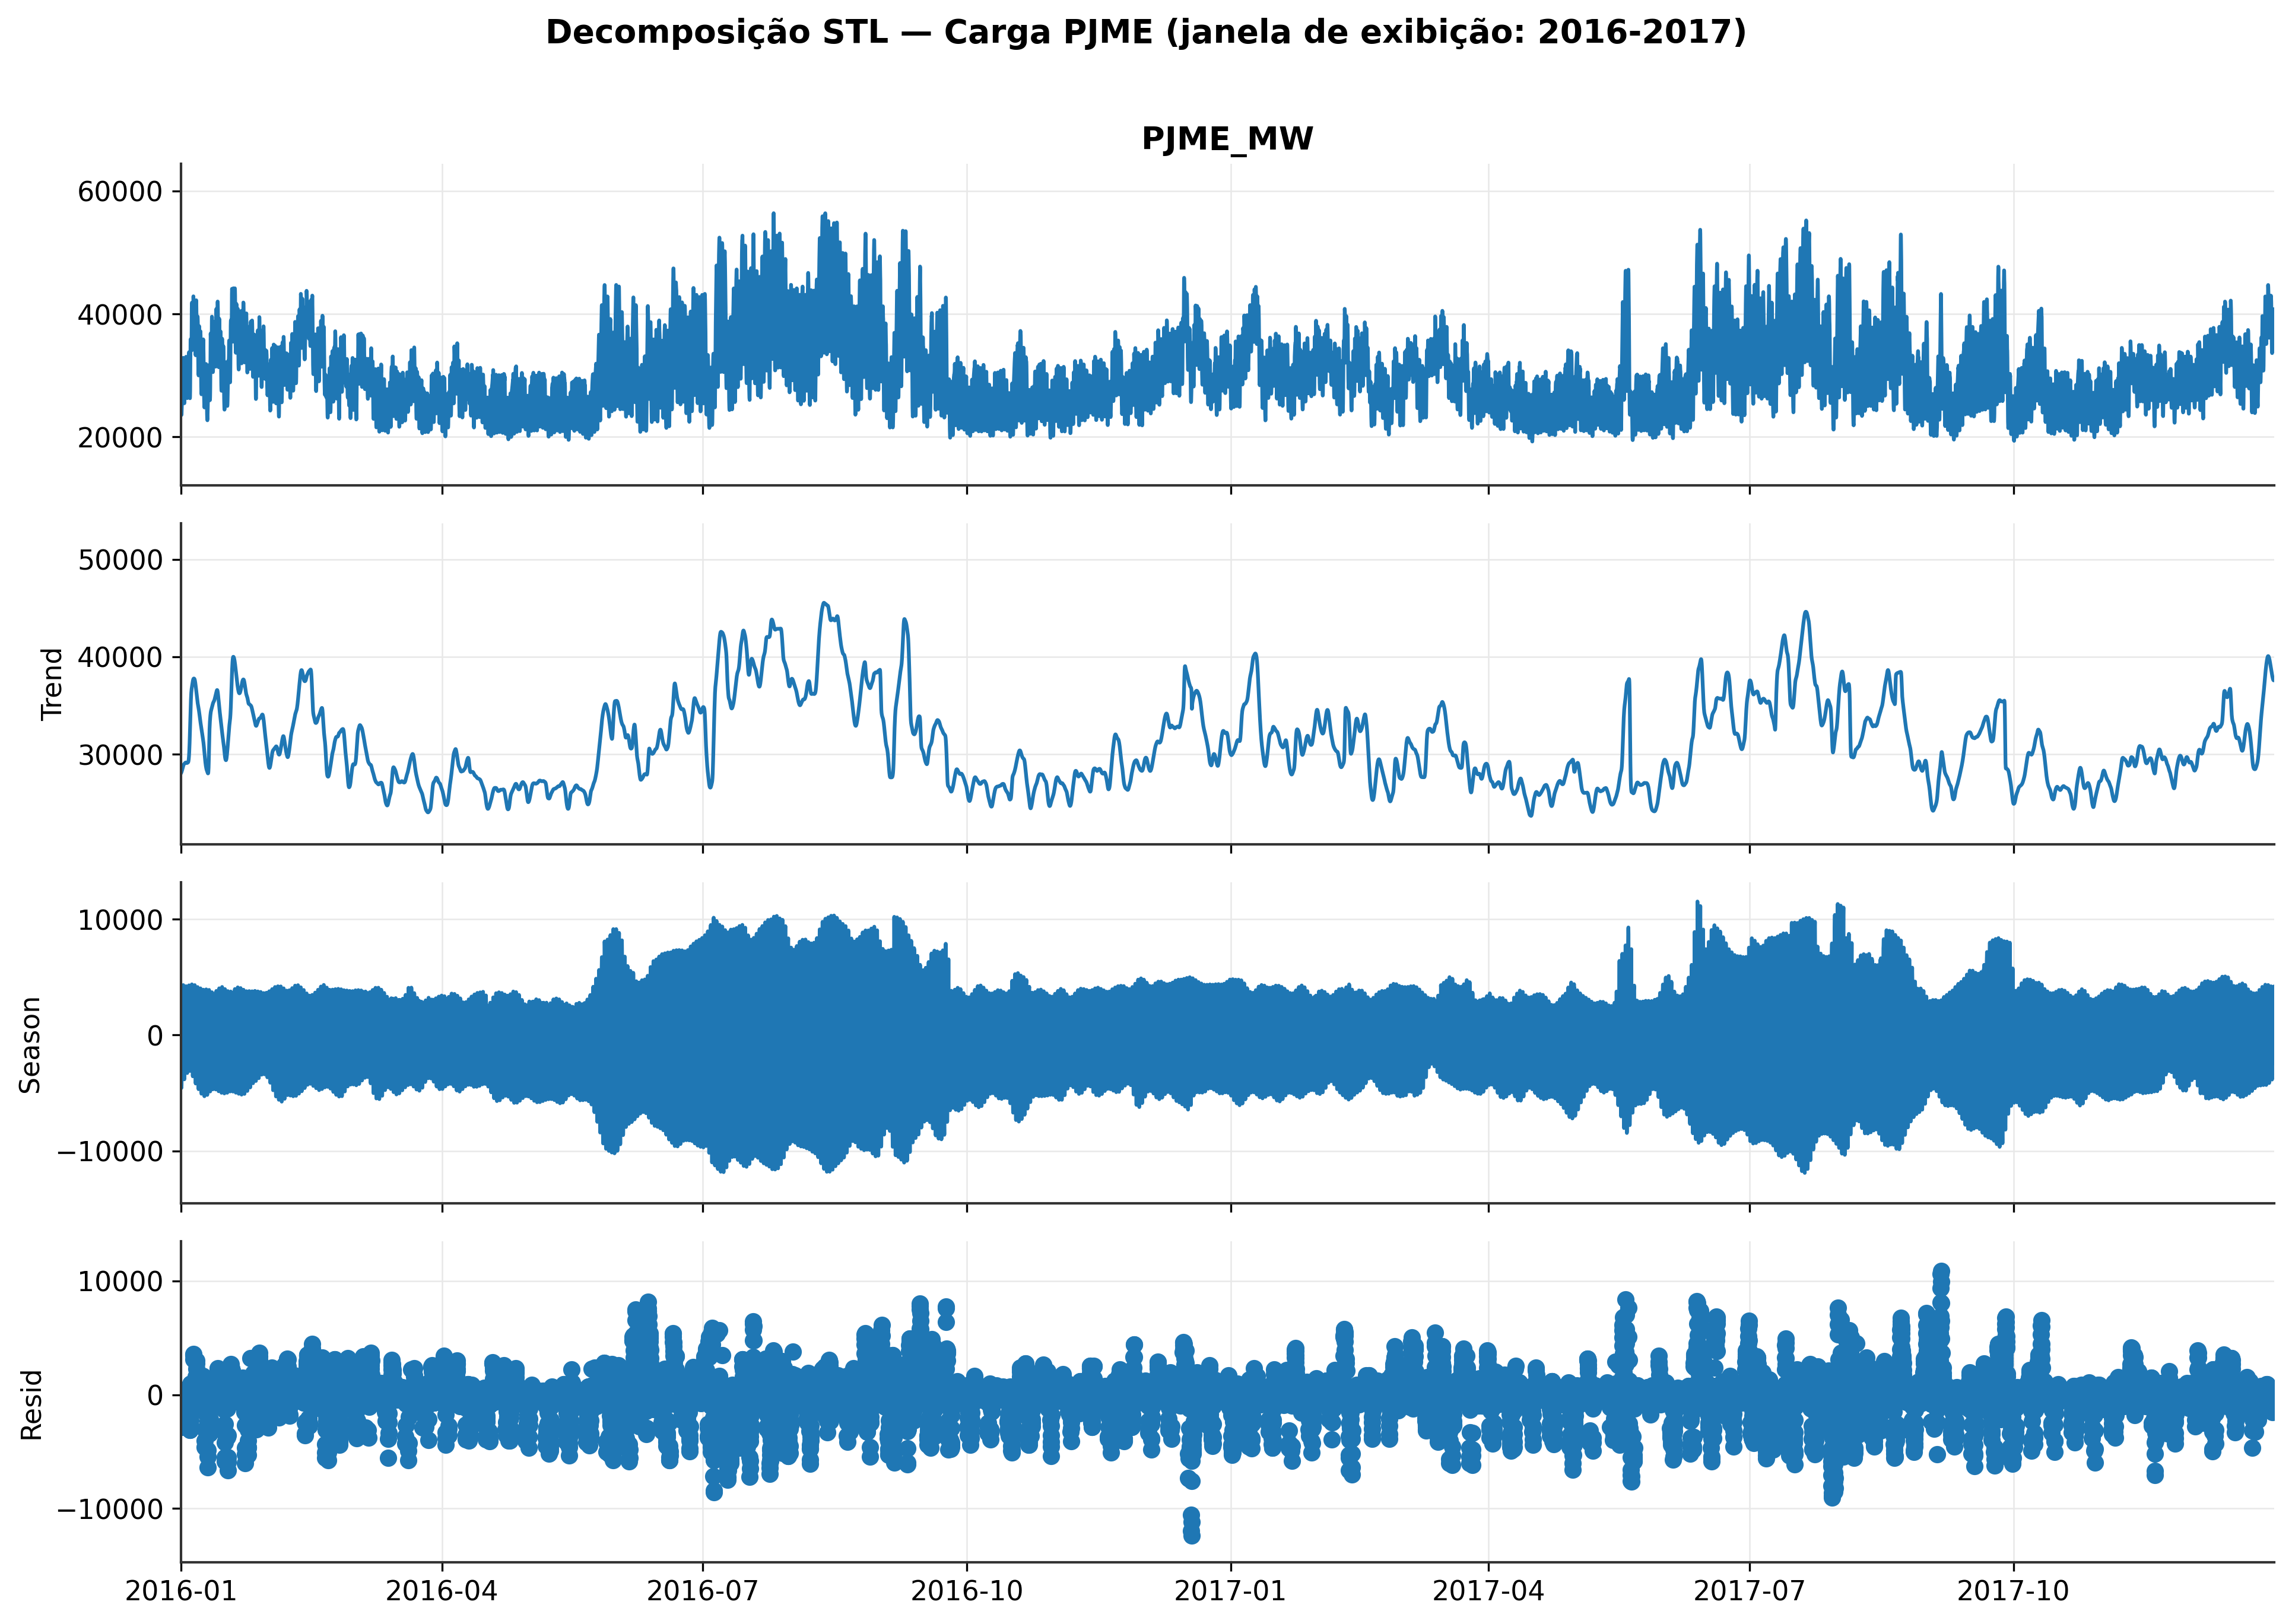
\includegraphics[width=0.85\textwidth]{Figuras_Aula3/fig3-decomposicao-stl.png}
    \caption{Decomposição STL: Carga PJME.}
    \label{fig:fig1}
\end{figure}


\newpage
% ============================================================
% EXERCÍCIO 2
% ============================================================
\section{Exercício 2: Padrões Cíclicos, Dependência Temporal e Relações Multivariadas}

\subsection{Padrões cíclicos: hora do dia, dia da semana e heatmap calendário}

\begin{figure}[H]
    \centering
    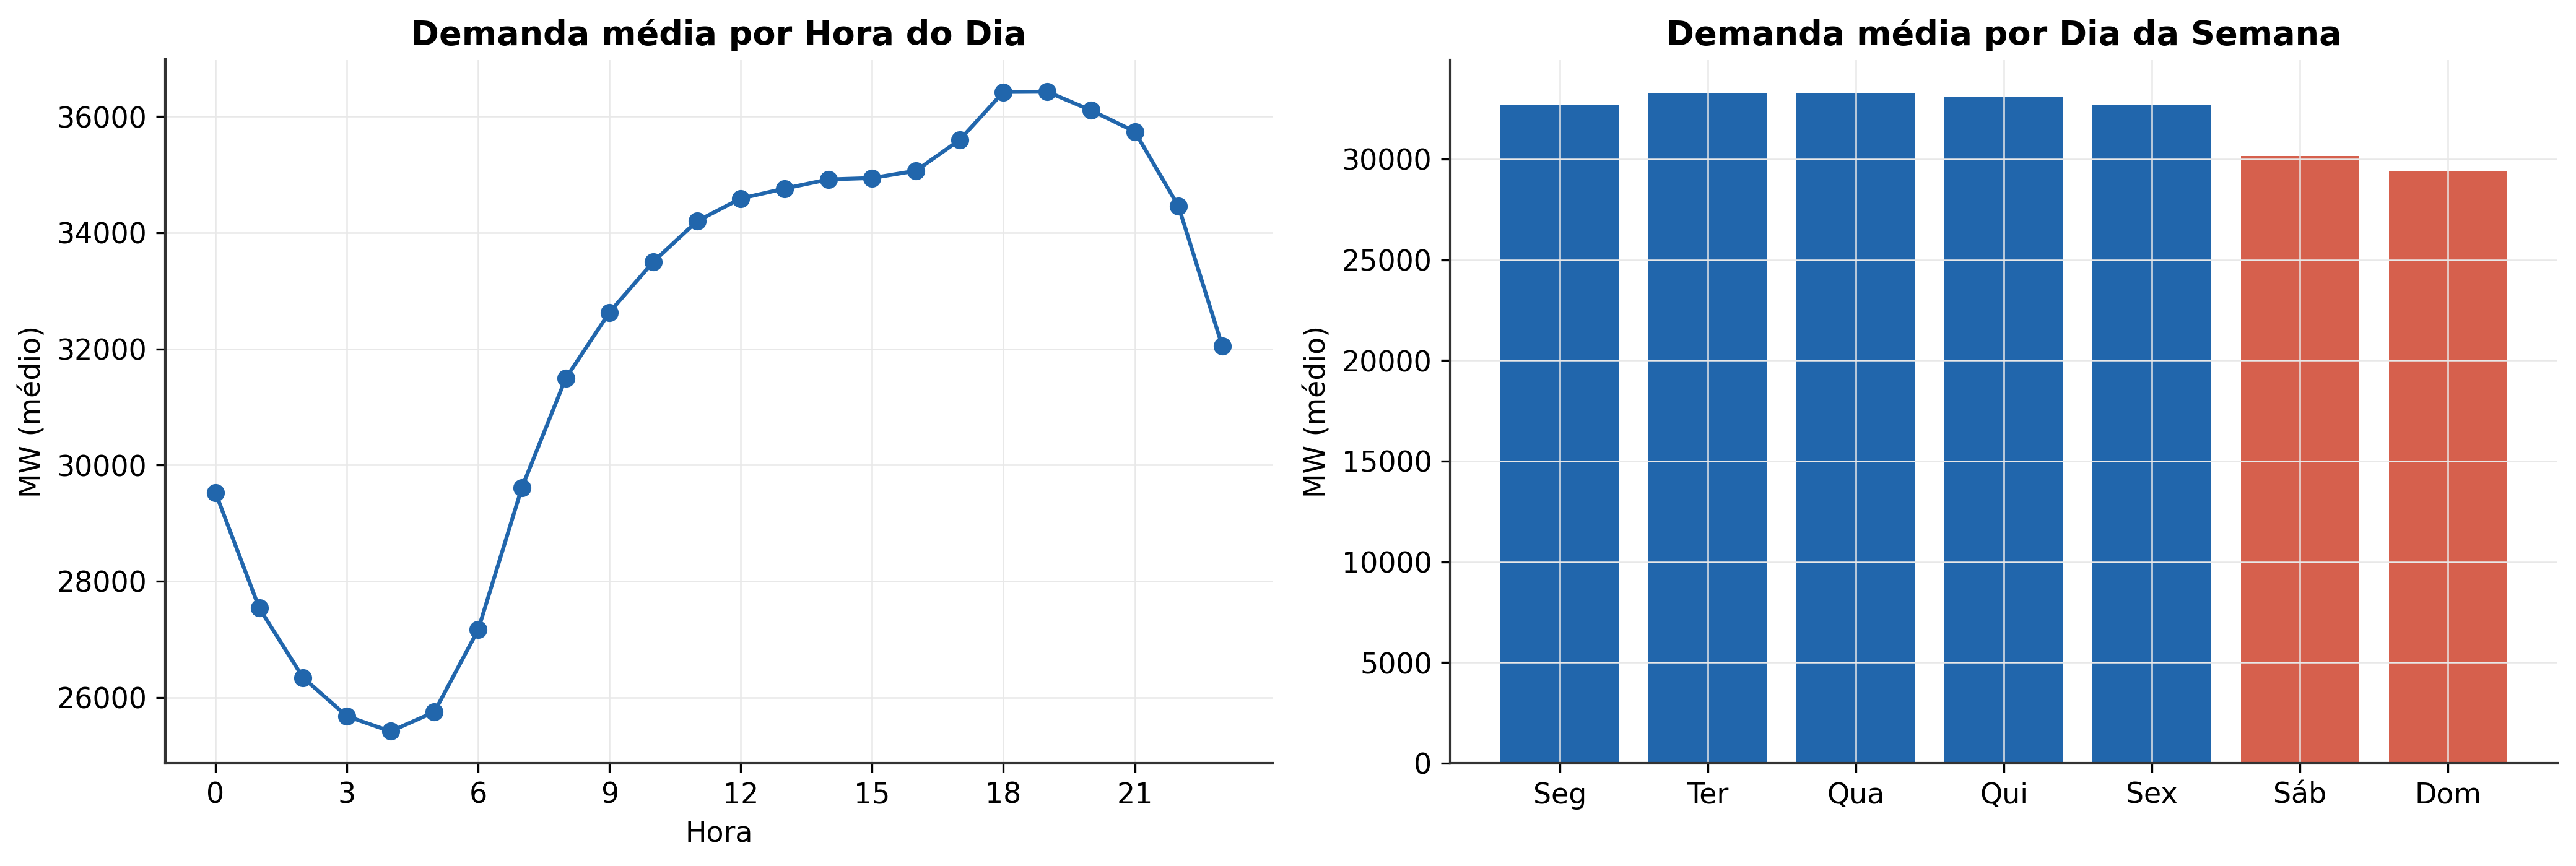
\includegraphics[width=0.85\textwidth]{Figuras_Aula3/fig4-perfil-hora-dia-semana.png}
    \caption{Padrões cíclicos: demanda média por hora e por dia da semana.}
    \label{fig:fig1}
\end{figure}

\noindent O perfil horário mostra dois "ombros" de maior demanda (manhã e final da tarde/noite), com vale de madrugada. O perfil semanal mostra queda visível de sábado e, principalmente, domingo.

\begin{figure}[H]
    \centering
    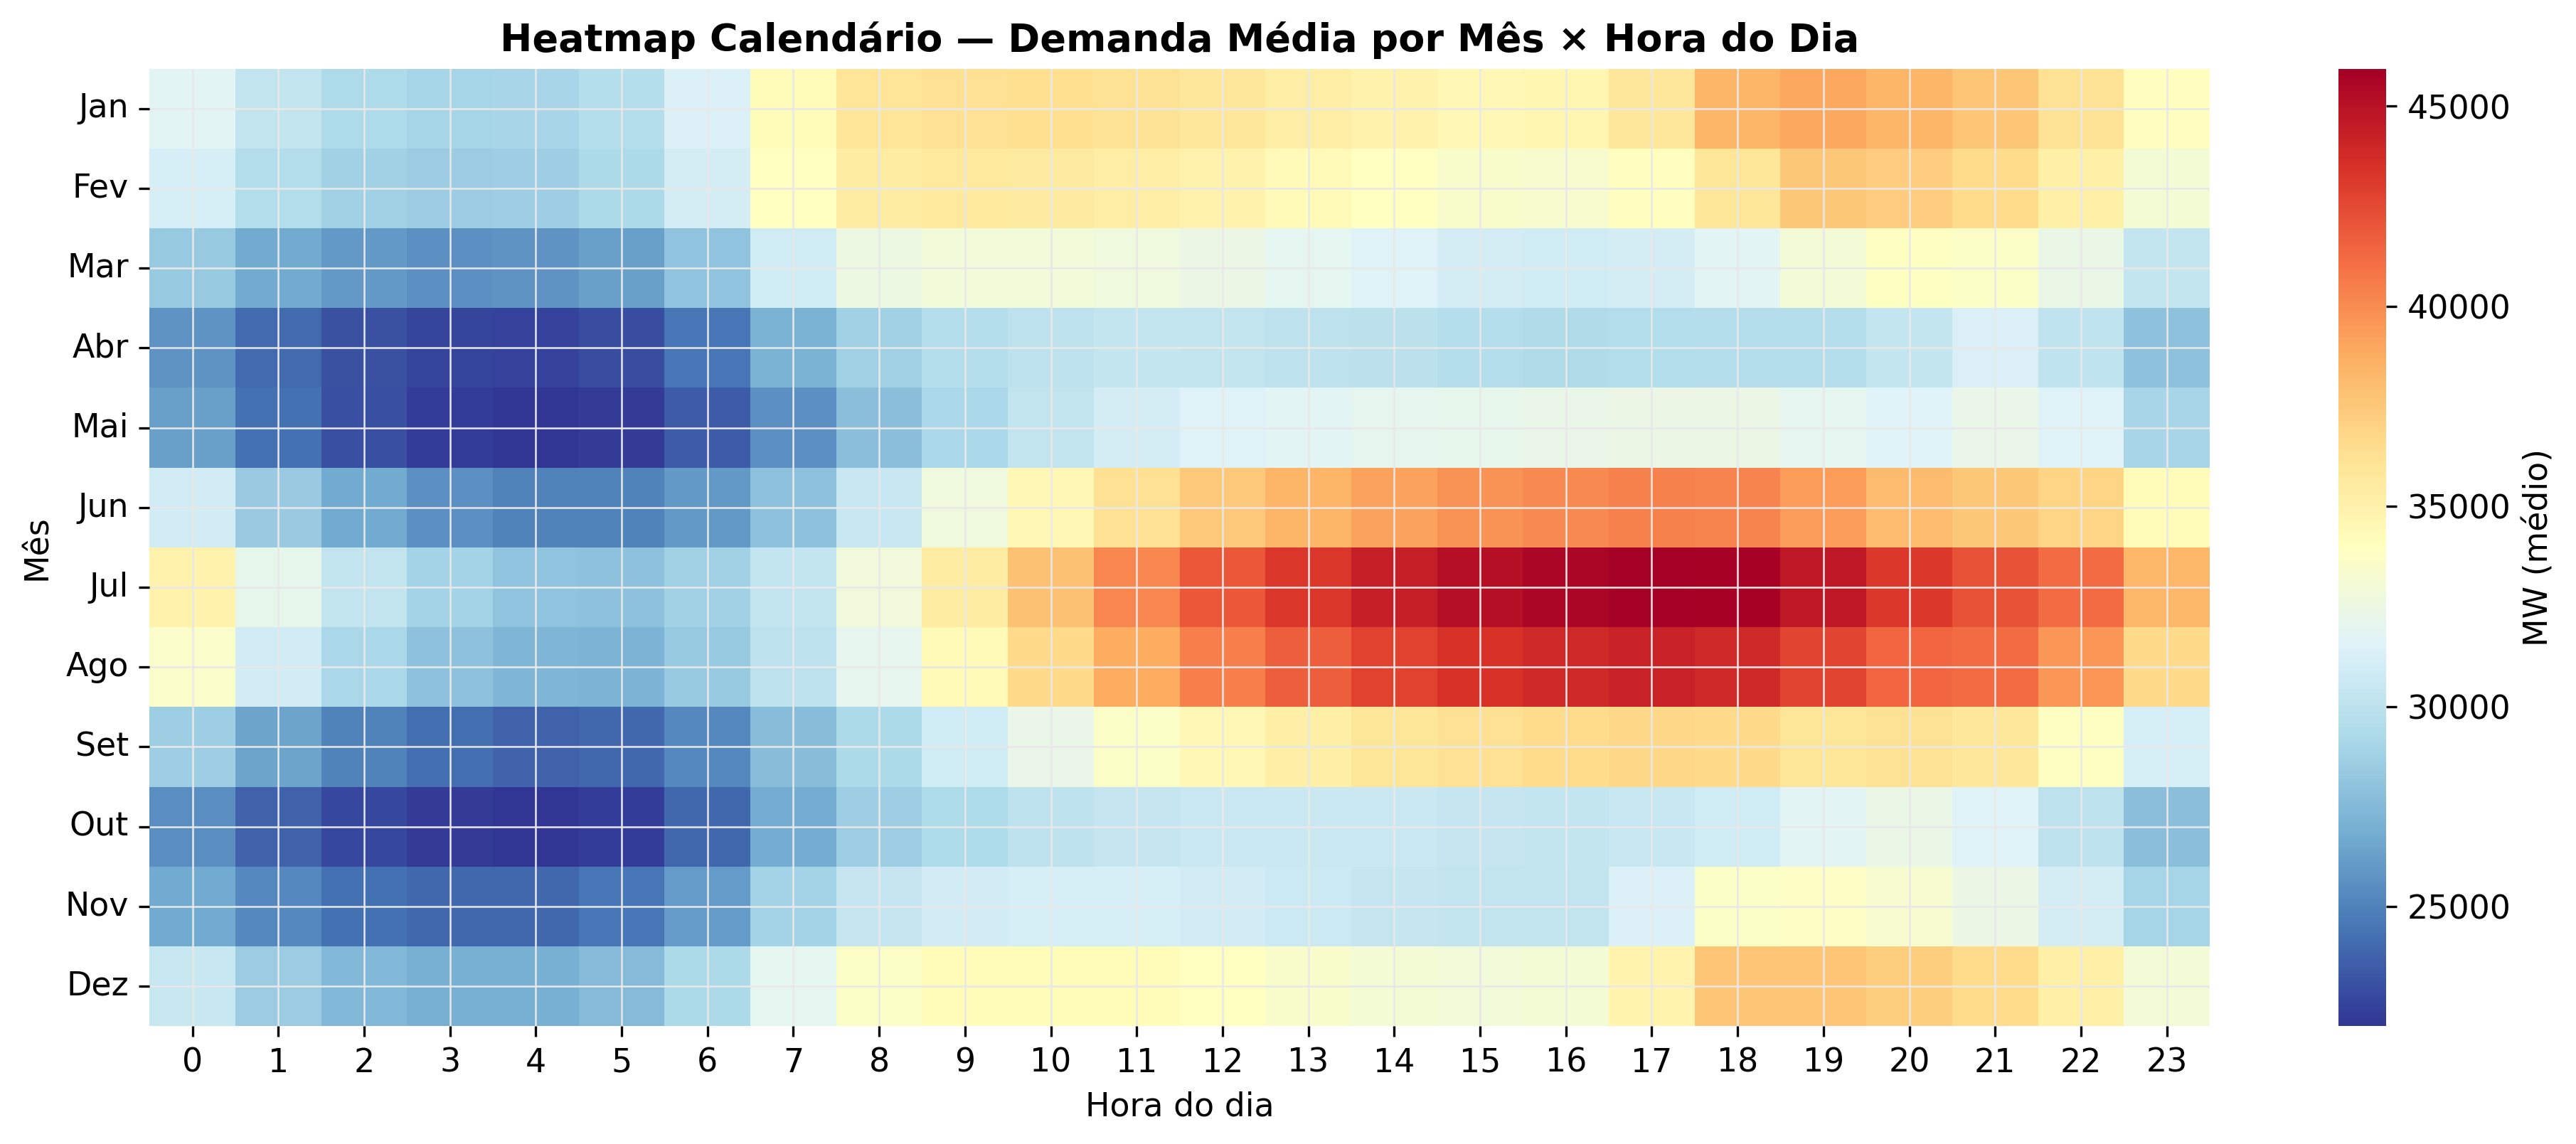
\includegraphics[width=0.85\textwidth]{Figuras_Aula3/fig5-heatmap-mes-hora.png}
    \caption{Heatmap calendário: demanda média por mês $\times$ hora do dia.}
    \label{fig:fig1}
\end{figure}


\noindent O heatmap revela que o formato do perfil horário muda com a estação: no verão (jun--ago) o pico se desloca para o início da noite (ar-condicionado no fim da tarde), enquanto no inverno (dez--fev) há dois picos mais definidos (manhã e noite, aquecimento), uma interação estação$\times$hora que um STL de sazonalidade única não captura.

\subsection{Autocorrelação (ACF) e Autocorrelação Parcial (PACF)}

\begin{figure}[H]
    \centering
    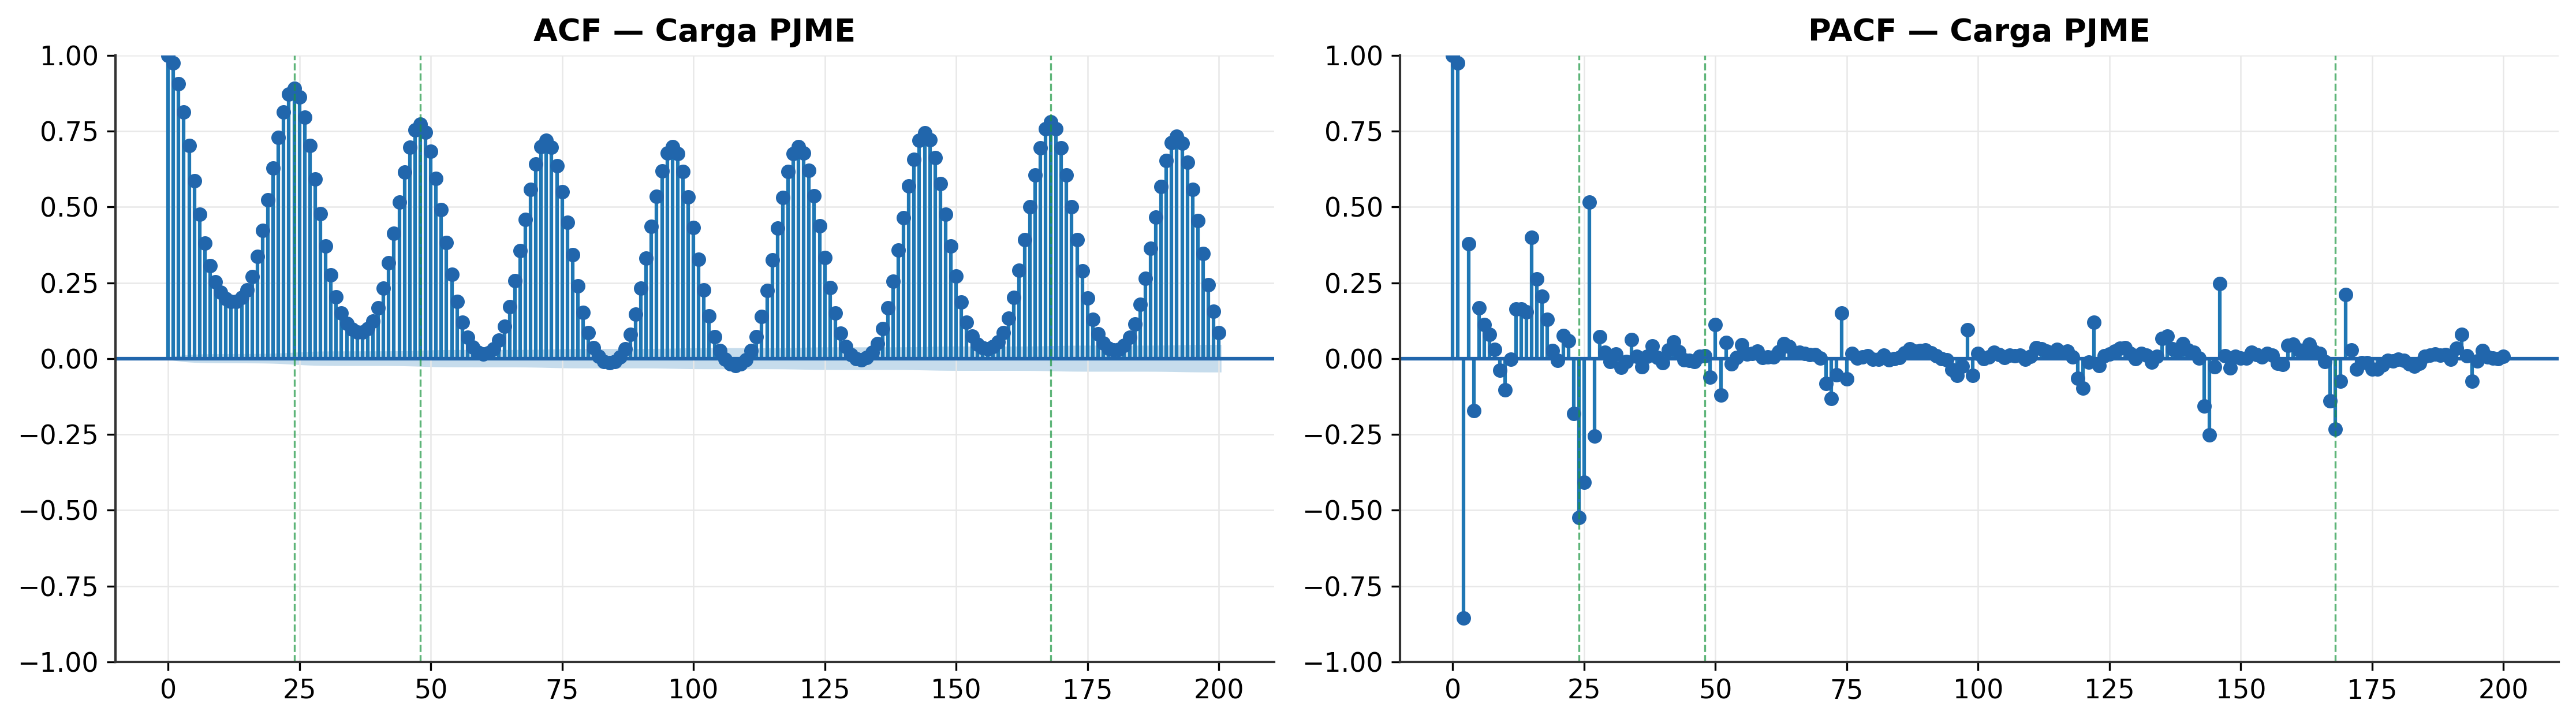
\includegraphics[width=0.85\textwidth]{Figuras_Aula3/fig6-acf-pacf.png}
    \caption{ACF/PACF: Carga PJME.}
    \label{fig:fig1}
\end{figure}

\noindent A ACF mostra decaimento lento com picos fortes e persistentes em múltiplos de 24h e em 168h (1 semana), dupla sazonalidade diária+semanal. A PACF cai mais rápido, mas ainda evidencia coeficientes relevantes nos lags 24 e 168.

\subsection{Espectro de Potência (FFT/Periodograma)}

\begin{table}[H]
\centering
\caption{Periodograma: períodos dominantes (série sem tendência)}
\begin{tabular}{lc}
\toprule
Período (horas) & Densidade espectral \\
\midrule
24{,}00 & $1{,}798\times10^{12}$ \\
12{,}00 & $2{,}938\times10^{11}$ \\
24{,}07 & $1{,}026\times10^{11}$ \\
23{,}93 & $7{,}690\times10^{10}$ \\
24{,}06 & $4{,}374\times10^{10}$ \\
\bottomrule
\end{tabular}
\end{table}

\begin{figure}[H]
    \centering
    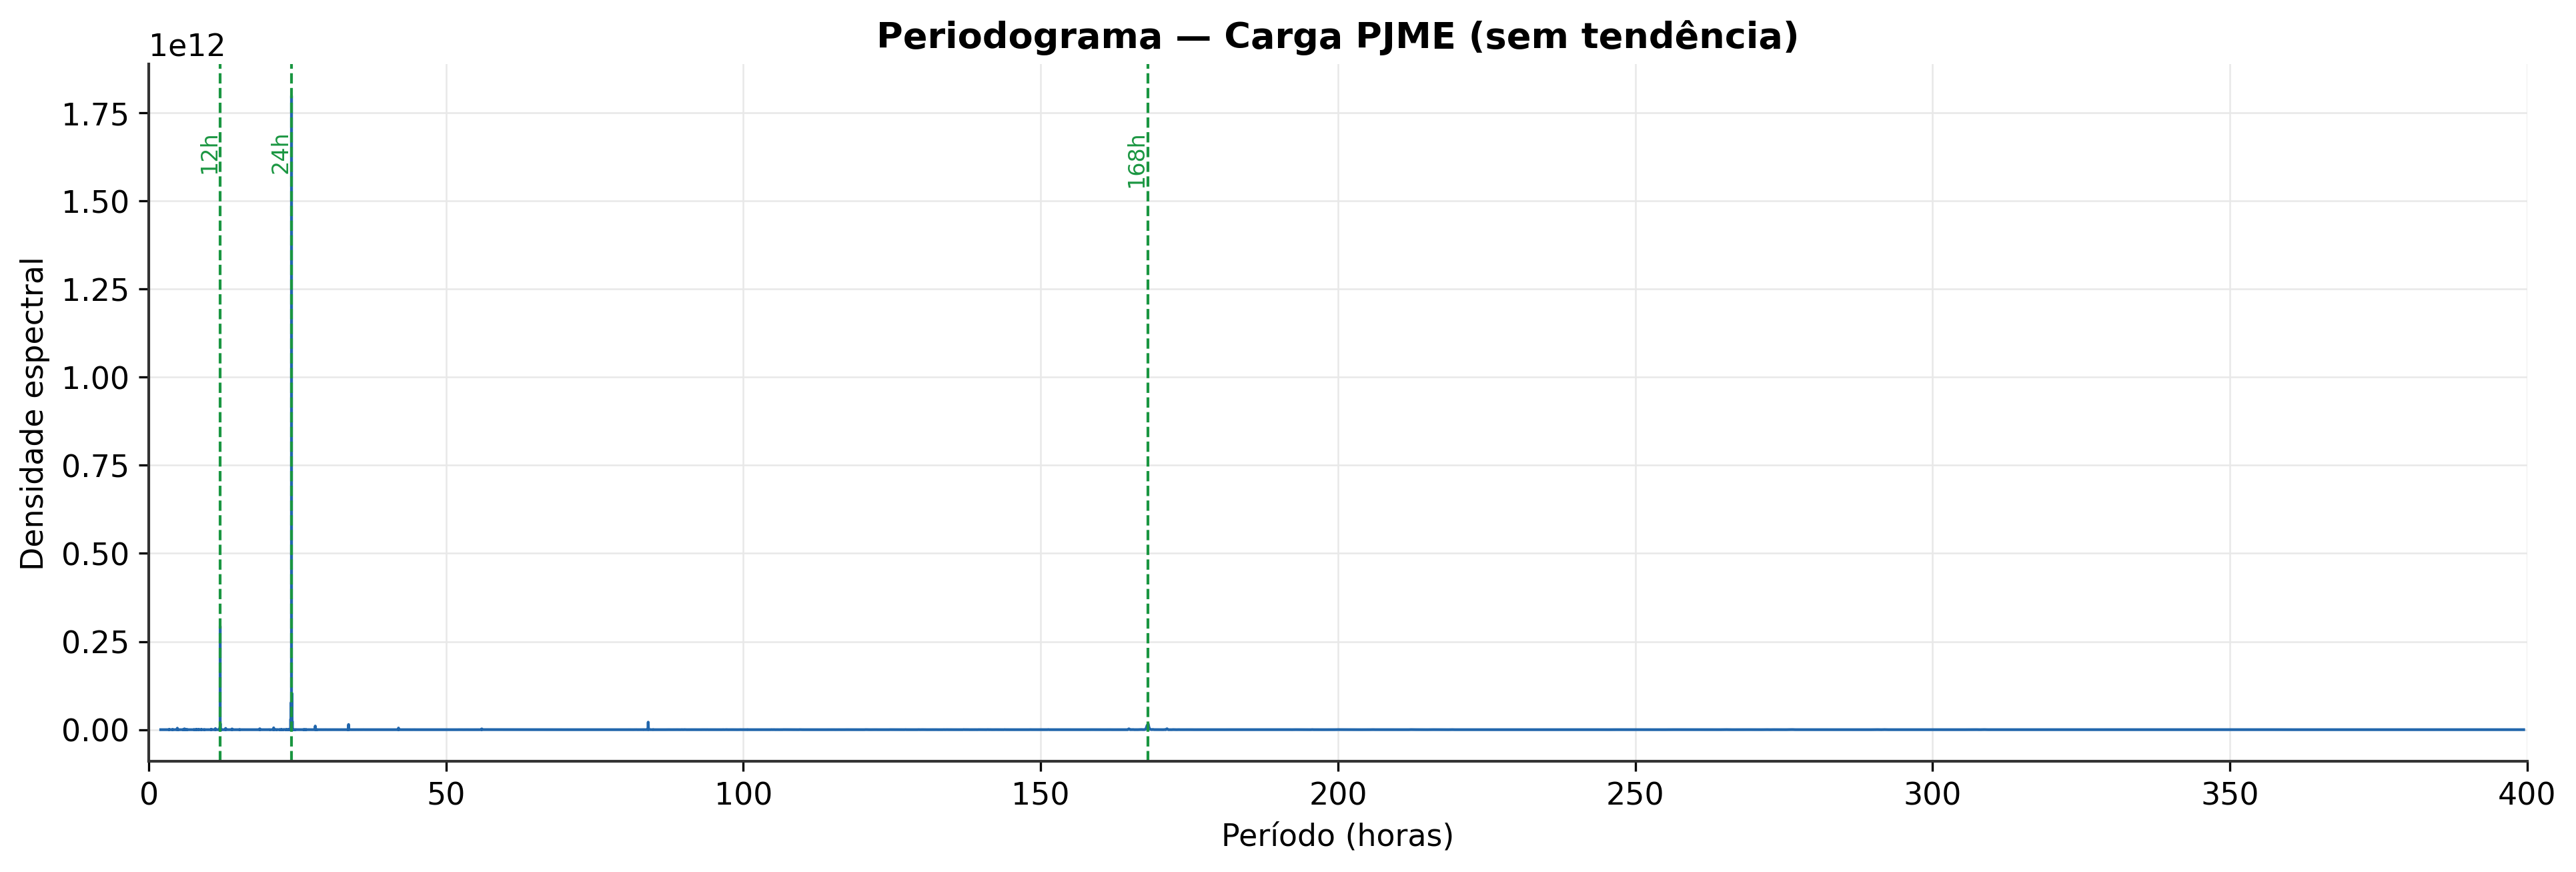
\includegraphics[width=0.85\textwidth]{Figuras_Aula3/fig7-periodograma.png}
    \caption{Periodograma: Carga PJME (sem tendência).}
    \label{fig:fig1}
\end{figure}

\noindent O periodograma confirma os mesmos picos da ACF/PACF: período dominante de 24h (ciclo diário), harmônico em 12h, e pico nítido em 168h (ciclo semanal), concordância entre os domínios do tempo e da frequência.

\subsection{Estacionariedade: Diagnóstico Combinado ADF + KPSS}

\begin{table}[H]
\centering
\caption{Diagnóstico combinado ADF + KPSS}
\begin{tabular}{lcccccc}
\toprule
Série & ADF stat & ADF $p$ & ADF estac.? & KPSS stat & KPSS $p$ & Veredito \\
\midrule
Bruta          & $-24{,}88$ & 0{,}0 & Sim & 3{,}54 & 0{,}01 & Conflito ADF$\times$KPSS \\
1ª diferença   & $-66{,}12$ & 0{,}0 & Sim & 0{,}0007 & 0{,}10 & Estacionária (concordam) \\
Resíduo STL    & $-48{,}33$ & 0{,}0 & Sim & 2{,}09 & 0{,}01 & Conflito ADF$\times$KPSS \\
\bottomrule
\end{tabular}
\end{table}

\noindent O conflito ADF$\times$KPSS na série bruta e no resíduo do STL é o padrão esperado para séries com sazonalidade determinística forte (sazonalidade semanal remanescente); a 1ª diferença satisfaz ambos os testes simultaneamente.

\subsection{Relações Bivariadas e Multivariadas}

\subsubsection*{10a. Correlação com variável exógena numérica (PJMW)}

\begin{table}[H]
\centering
\caption{Correlação PJME (alvo) vs. PJMW (exógena numérica)}
\begin{tabular}{lcc}
\toprule
Coeficiente & Valor & $p$-valor \\
\midrule
Pearson $r$    & 0{,}8757 & $<10^{-300}$ \\
Spearman $\rho$ & 0{,}8890 & $<10^{-300}$ \\
Kendall $\tau$  & 0{,}7085 & $<10^{-300}$ (amostra de 20.000 pontos) \\
\bottomrule
\end{tabular}
\end{table}

\subsubsection*{10b. Variável categórica natural: Tipo de Dia (Dia útil vs. Fim de semana)}

\begin{table}[H]
\centering
\caption{Tabela de contingência: Faixa de Demanda $\times$ Tipo de Dia}
\begin{tabular}{lcc}
\toprule
Faixa de demanda & Dia útil & Fim de semana \\
\midrule
Baixa  & 27.185 & 21.285 \\
Média  & 36.817 & 11.642 \\
Alta   & 39.870 &  8.593 \\
\bottomrule
\end{tabular}
\end{table}

\noindent Qui-quadrado: $\chi^2=8874{,}7$, $\text{dof}=2$, $p<10^{-300}$, rejeita fortemente $H_0$ de independência: fins de semana concentram muito mais observações na faixa "Baixa".

\begin{table}[H]
\centering
\caption{Teste $t$, Demanda: Dia útil vs. Fim de semana}
\begin{tabular}{lc}
\toprule
Grandeza & Valor \\
\midrule
Média dia útil ($n=103.872$)     & 32.996,1 MW \\
Média fim de semana ($n=41.520$) & 29.784,4 MW \\
Teste $t$                        & $t=93{,}1$, $p<10^{-300}$ \\
Cohen's $d$                      & 0{,}510 (efeito médio) \\
\bottomrule
\end{tabular}
\end{table}

\begin{table}[H]
\centering
\caption{ANOVA: Demanda por Estação do Ano (Hemisfério Norte)}
\begin{tabular}{lccc}
\toprule
Estação & Média (MW) & Desvio-padrão & $n$ \\
\midrule
Inverno    & 33.503,1 & 4.665,9 & 36.071 \\
Outono     & 29.626,2 & 5.183,3 & 34.944 \\
Primavera  & 29.034,9 & 4.607,5 & 37.536 \\
Verão      & 36.112,5 & 7.942,5 & 36.841 \\
\bottomrule
\end{tabular}
\\[0.2cm]
\footnotesize{$F=12.309{,}4$, $p<10^{-300}$, $\eta^2=0{,}2026$ (efeito grande).}
\end{table}

\subsubsection*{Informação Mútua}

\begin{table}[H]
\centering
\caption{Informação mútua: variáveis exógenas vs. demanda (PJME)}
\begin{tabular}{lc}
\toprule
Variável & Informação Mútua \\
\midrule
PJMW           & 0{,}8321 \\
hora           & 0{,}2862 \\
estacao\_cod   & 0{,}1504 \\
dia\_semana    & 0{,}0407 \\
tipo\_dia\_cod & 0{,}0346 \\
\bottomrule
\end{tabular}
\end{table}

\noindent A carga da região vizinha (PJMW) e a hora do dia concentram a maior informação mútua com a demanda-alvo, coerente com a forte correlação linear e o forte ciclo diário observados acima.

\subsection{Detecção de anomalias por Z-score móvel vs. outliers estáticos}

\begin{table}[H]
\centering
\caption{Anomalias: Z-score móvel (janela=48h, sobre resíduo do STL) vs. outliers estáticos}
\begin{tabular}{lcc}
\toprule
Método & Nº de pontos & \% dos dados \\
\midrule
Z-score móvel ($|z|>3{,}0$) & 995 & 0{,}684\% \\
IQR (estático)               & 3.460 & 2{,}380\% \\
MAD (estático)                & 1.003 & 0{,}690\% \\
\midrule
Só pelo Z-score móvel (não capturados pelos estáticos) & \multicolumn{2}{c}{983} \\
Z-score móvel + pelo menos um método estático          & \multicolumn{2}{c}{12} \\
\bottomrule
\end{tabular}
\end{table}

\begin{figure}[H]
    \centering
    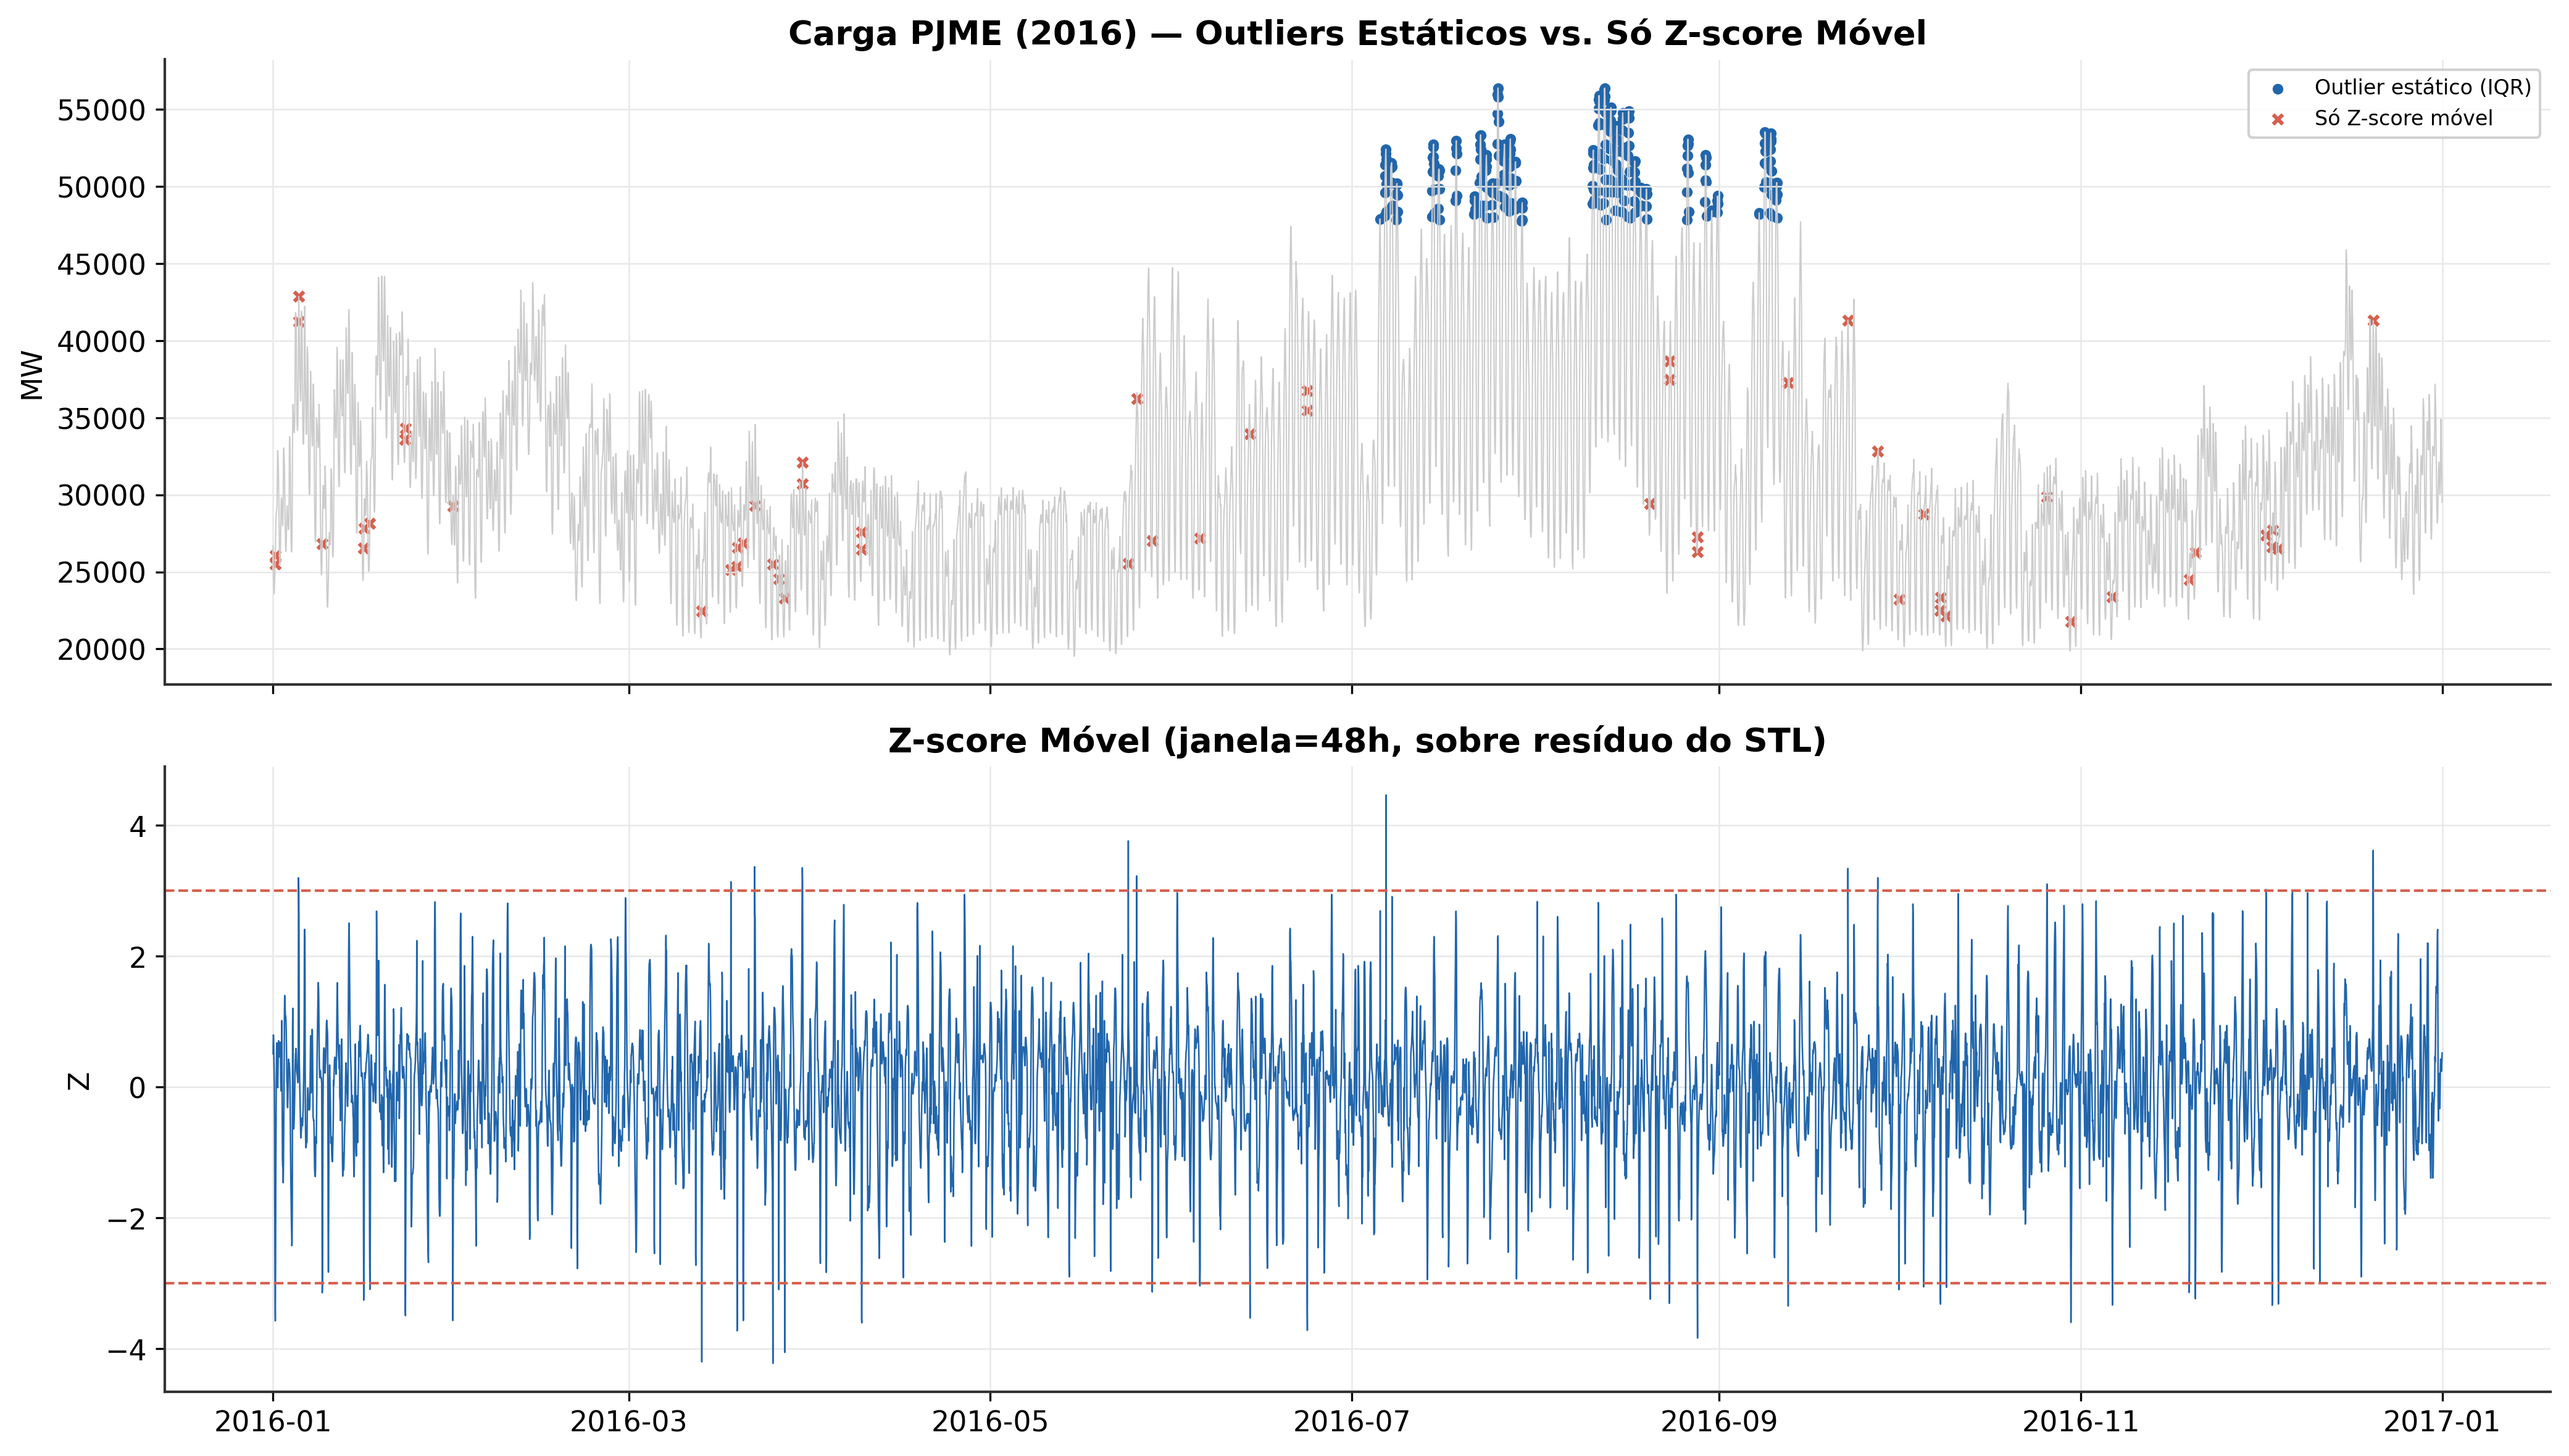
\includegraphics[width=0.85\textwidth]{Figuras_Aula3/fig8-anomalias-zscore-movel.png}
    \caption{Anomalias: Z-score móvel vs. outliers estáticos.}
    \label{fig:fig1}
\end{figure}

\noindent \textbf{Nota técnica:} aplicar o z-score móvel diretamente sobre a série \emph{bruta} se mostrou inadequado, o desvio-padrão de uma janela de 48h sobre a série bruta já incorpora a própria oscilação do ciclo diário como "variação normal", inflando o denominador e escondendo quase todas as anomalias reais (nenhum ponto ultrapassava $|z|>3$ mesmo em dias de pico extremo). Por isso, o z-score móvel foi aplicado sobre o \textbf{resíduo do STL} (já sem tendência nem sazonalidade diária), isolando corretamente os desvios anômalos locais: 983 dos 995 pontos sinalizados não haviam sido capturados pelos métodos estáticos (IQR/MAD), evidenciando que esses métodos capturam fenômenos complementares, picos sazonais globais (estáticos) vs. mudanças de regime locais (z-score móvel).

\subsection{Tabela-Síntese: EDA $\rightarrow$ Decisões de Modelagem}

\begin{table}[H]
\centering
\small
\begin{tabular}{p{6.5cm}p{7.5cm}}
\toprule
\textbf{Achado da EDA} & \textbf{Decisão de modelagem} \\
\midrule
Duplicatas/lacunas ligadas ao DST, padrão MCAR determinístico & Consolidar duplicatas e interpolar lacunas antes de qualquer modelagem \\
Distribuição assimétrica; normalidade fortemente rejeitada & Evitar assumir erros gaussianos; considerar MAE/Huber ou transformação \\
Outliers de consenso concentrados em maio--set. (ondas de calor) & Não remover, sinalizar como \emph{feature} de evento extremo \\
$F_S$ muito alta; $F_T$ moderada/alta & Modelar sazonalidade diária explicitamente (Fourier/dummies horárias) \\
Heatmap mês$\times$hora mostra interação estação$\times$hora & Incluir termos de interação hora$\times$mês/estação \\
ACF/PACF e FFT concordam: picos em 24h, 12h e 168h & Usar lags 24/48/168; considerar MSTL (múltiplas sazonalidades) \\
ADF$\times$KPSS conflitam na bruta, concordam na diferença/resíduo & Diferenciar a série (ou usar resíduo do STL) antes de modelos estacionários \\
Correlação forte com PJMW (Pearson/Spearman/Kendall altos) & Incluir a carga da região vizinha como covariável exógena \\
Qui-quadrado, teste $t$ e ANOVA confirmam dependência de tipo de dia/estação & Incluir tipo de dia e estação/mês como variáveis categóricas fortes \\
Informação mútua mais alta em PJMW e hora & Priorizar essas variáveis na engenharia de atributos \\
Z-score móvel (resíduo STL) captura anomalias locais que os métodos estáticos não capturam & Usar detecção de anomalia por janela local sobre o resíduo em produção \\
\bottomrule
\end{tabular}
\caption{Síntese da EDA às decisões de modelagem (PJM Hourly Energy Consumption)}
\end{table}

\newpage
% ============================================================
% CONCLUSÃO GERAL
% ============================================================
\section{Considerações Finais}

Os dois exercícios, aplicados sobre o mesmo dataset real, ilustram como um roteiro completo de EDA orienta decisões concretas de modelagem: a qualidade dos dados revelou um mecanismo determinístico de dados ausentes (DST); a análise univariada e de outliers indicou a necessidade de perdas/métricas robustas e o tratamento diferenciado de anomalias sazonais reais; e a análise cíclica, de autocorrelação, de frequência e de estacionariedade convergiram para o mesmo diagnóstico, uma \textbf{dupla sazonalidade} (diária e semanal) que exige tratamento explícito (múltiplas sazonalidades ou termos de Fourier) em qualquer modelo de previsão. Por fim, a análise multivariada confirmou estatisticamente (correlação, qui-quadrado, teste $t$, ANOVA e informação mútua) que região vizinha, hora do dia, tipo de dia e estação do ano são todas covariáveis relevantes a incluir em um modelo preditivo.

\end{document}